
\section{Experiments}
\label{sec:experiments}

This section is composed of two parts. First, the experimentation focuses on
the influence of the number of collaborators on the size of LSEQ and \NAME{}
identifiers.  A set of synthetic collaborators generates a document by
successively performing insert operations at the end. This experiment aims to
show the behaviour of the two strategy choices, and put the results in relation
with the expected sub-linear space complexity.

The second part of experiments consists in highlighting the effect of latency
on a document edited by multiple users. Once again, it aims to compare LSEQ and
\NAME{} and to show the impact of concurrency on the average size of
identifiers in the document.

The experiments focus on the digit bit-length of generated identifiers.
Indeed, all variable-size CRDTs rely on source and clock to guarantee the
unicity of identifiers, nevertheless, the space complexity mainly depends on
the digit choice made by the allocation strategy.

To perform these experiments, we implemented a simulation framework called
\emph{HumbleSimulator}. The sources are available on the Github platform under
the terms of the GPL
licence\footnote{\url{https://github.com/Chat-Wane/HumbleSimulator}}.

\subsection{Multiple users experiment}

\begin{asparadesc}
\item[Objective:] show that the random strategy choice without taking into
  account the strategies employed by other collaborators leads to a quick
  growth in the size of identifiers. On the opposite, when all collaborators
  uses a common allocation strategy at a given depth, the space complexity
  remains sub-linearly upper-bounded.

\item[Description:] we experiment LSEQ and \NAME{} with two different number of
  users. Thus, the setups are
  \begin{inparaenum}[(i)]
  \item a random strategy choice (\textbf{rand}) and
  \item a hash strategy choice (\textbf{hash}).
  \end{inparaenum}
  Both of these setups use \emph{boundary+} and \emph{boundary--} and have
  similar variable values $boundary=10$ and $base=2^{4+depth}$. A set of 10
  collaborators produces a document of 100 lines by performing 10 insert
  operations each.

\item[Results:] Figure~\ref{im:tenusers} shows on the top part the spectrum of
  the synthetic document, i.e., the revision date of each line. Since the bars
  are getting taller when they are closer of the end of the document, it
  indicates that the users edited at the end monotonically. On the second part
  of the Figure~\ref{im:tenusers}, we measure the identifier bit-length
  associated to each line. We observe that the identifiers of \textbf{rand}
  setup quickly increase while the \textbf{hash} identifiers remain similar as
  experiment made with one user in~\cite{nedelec2013lseq}. Consequently, the
  \textbf{hash} setup is the most suitable setup in the context of distributed
  collaborative editing.

\item[Reasons:] both setups use \emph{boundary+} and \emph{boundary--}
  allocation strategies. However, each collaborator in the \textbf{rand} setup
  makes independent choices of allocation strategies when required. Thus, when
  a collaborator chooses a particular strategy, and any other user chooses the
  antagonist strategy, and then the respective operations are delivered too
  each other, a large number of identifiers is wasted. On the other hand, when
  the same hash function spread over all collaborators generates the same
  strategy choices, it keeps the random behaviour locally and also makes an
  implicit agreement on which strategy to employ at a given depth.
\end{asparadesc}

\begin{figure}
\centering
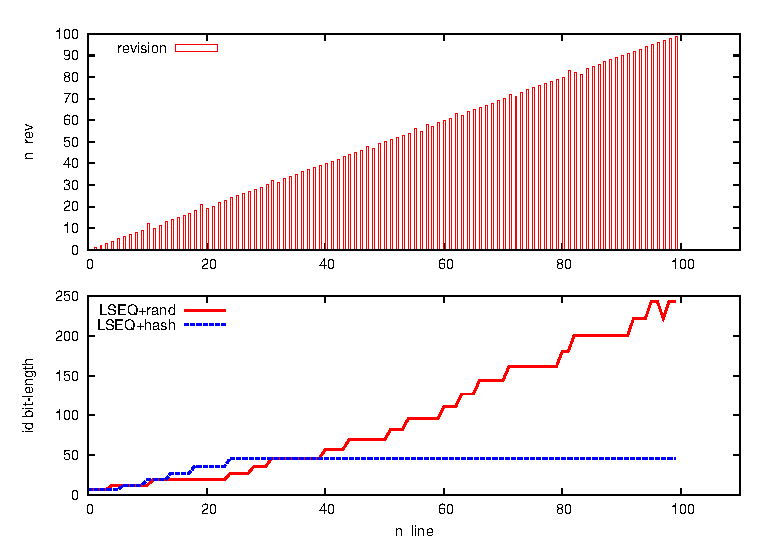
\includegraphics[width=0.49\textwidth]{img/tenusers.eps}
\caption{Experiments on a synthetic document of 100 lines edited at the end by
  10 collaborators (10 operations per user). The top figure shows the revision
  number of the operation. The bottom figure shows the bit-length of each
  identifier allocated to each line. On average, the bit-length of LSEQ and
  \NAME{} identifiers are 94.7 and 39.1 bit/id respectively.}
\label{im:tenusers}
\end{figure}


\subsection{Latency experiment}
\begin{asparadesc}
\item[Objective:] show that increasing the latency (the time between the
  generation and the delivery of an operation) does not imply a growth in the
  size of identifiers. On the contrary, when the latency increases, the average
  size of allocated identifiers decreases. This behaviour is expected on both
  LSEQ and \NAME{} that use a random strategy choice and a hash strategy choice
  respectively.
\item[Description:] we simulate a set of 10 collaborators producing a document
  of 100 lines. Each one of these collaborators performs 10 insert operations
  at the end of the document. The users generate operations following the
  Poisson distribution of parameter $\lambda=100$. i.e. users more likely
  generate an operation after 100 rounds (arbitrary unit) from their previous
  operation. Measurements are done at a latency of 5, 10, 20, 40, 80, 160, 320,
  640 rounds. They concern the average bit-length of identifiers in the
  document.  We evaluate two setups: the random strategy choice \textbf{rand}
  and the hash strategy choice \textbf{hash} using the allocation strategies
  $boundary+$ and $boundary-$ with $boundary=10$ and departure
  $base=2^{4+depth}$.
\item[Results:] Figure~\ref{im:stats} shows the results of the latency
  experiments. As expected, the two setups allocate identifiers with an average
  bit-length that quickly decreases when the latency increases. Therefore, the
  latency does not badly affect LSEQ and \NAME{} allocation strategies. Also,
  it confirms observations made in previous experiment: \textbf{hash} performs
  better than \textbf{rand} especially on low latency.
\item[Reasons:] increasing the latency delays the arrival of operations to the
  remote collaborators. Thus, each collaborator works locally until it delivers
  the operation generated by other users. Considering the extreme case with the
  maximum latency, each collaborator generates its 10 insertions, and then
  merges the others' 90 operations. Consequently, the 100 operations share the
  same space, i.e., the digit part of identifiers can be the same for multiple
  elements, and the total order is maintained by the source and clock.
\end{asparadesc}


\begin{figure}
\begin{center}
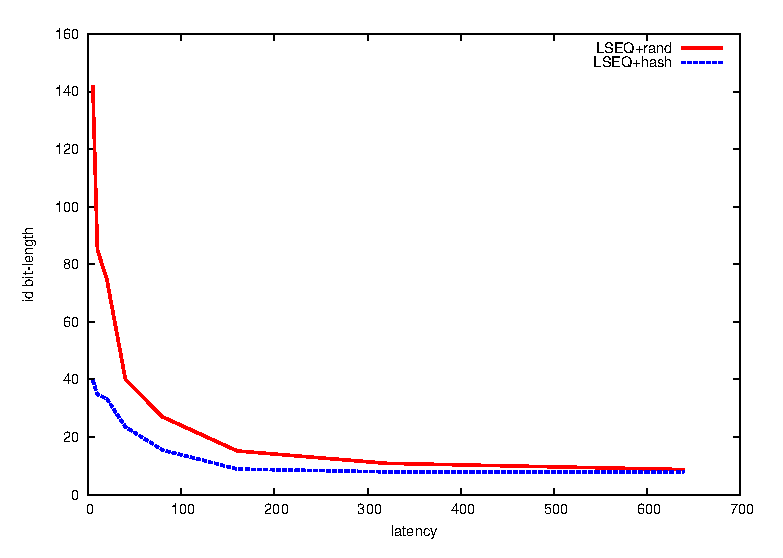
\includegraphics[width=0.49\textwidth]{img/stats.eps}
\caption{Experiments of latency effects over the average bit-length of
  identifiers. A group of 10 collaborators generates a synthetic document of
  100 lines (10 operations each). Two configurations of LSEQ: the original
  random strategy choice and the hash strategy choice (\NAME{}).}
\label{im:stats}
\end{center}
\end{figure}

\subsection{Synthesis}
The experiments evaluated the effect of concurrency on the average bit-length
of identifiers by varying the number of collaborators and the latency. They
showed that an implicit and \emph{a priori} agreement on allocation strategy
choices is required to maintain the sub-linear upper-bound on space
complexity. Employing the same hash function to chose the allocation strategy
permits to reach this agreement. Consequently, the improvement of LSEQ called
\NAME{} can be safely used in distributed collaborative editing. The latency
experiment shows that increasing the latency parameter only results in sharing
the identifier space, and consequently lowers the size of identifiers. As a
corollary, considering an immediate delivery of operations constitutes a
sufficient upper-bound on the behaviour of the overall system under higher
latency.

%%% Local Variables: 
%%% mode: latex
%%% TeX-master: "../dchanges"
%%% End: 
